\usetikzlibrary{shapes}

\chapter{Semantics}

%%%%%%%%%%%%%%%%%%%%%%%%%%%%%%%%%%%%%%%%%%%%%%%%%%%%%%%%%%%%%%%%%%%%%%%%%%%%%%%
\section{Denotational Semantics}

\[
\Denot{\cdot} \colon
  \syncatset{Term} \times (\syncatset{Var} \rightarrow \mathcal{D})
    \rightarrow \mathcal{D}_{\bot}
\]

\begin{alignat*}{2}
  \Denot{x}_\rho & = \rho(x) \\
  \Denot{\lambda x.t}_\rho & =
    \psi(\mathbf{\lambda} v. \Denot{t}_{\rho [x \mapsto v]}) \\
  \Denot{t_1 \; t_2}_\rho & =
    \varphi(\Denot{t_1}_\rho) \Denot{t_2}_\rho
\end{alignat*}

%%%%%%%%%%%%%%%%%%%%%%%%%%%%%%%%%%%%%%%%%%%%%%%%%%%%%%%%%%%%%%%%%%%%%%%%%%%%%%%
\section{Expressions, Values, and Operational Semantics}

\begin{alignat*}{2}
  e & \Coloneqq v \mid e\;e         \tag{expressions} \\
  v & \Coloneqq \lambda x.e \mid x  \tag{values}
\end{alignat*}

%%%%%%%%%%%%%%%%%%%%%%%%%%%%%%%%%%%%%%%%%%%%%%%%%%%%%%%%%%%%%%%%%%%%%%%%%%%%%%%
\section{Structural Operational Semantics}

We can classify evaluation rules to:
\begin{itemize}
    \item reduction rules, which do computations (e.g. application rule below)
    \item structural congruence rules, which indicate when and which subterms can be evaluated;
        they define evaluation order
\end{itemize}

\begin{mathpar}
  \inferrule{\phantom{e}}
            {(\lambda x.e)\;v \longrightarrow e\{v/x\}}
  
  \inferrule{e_1 \longrightarrow e_1'}
            {e_1 \; e_2 \longrightarrow e_1' \; e_2}

  \inferrule{e \longrightarrow e'}
            {v \; e \longrightarrow v \; e'}
\end{mathpar}

%%%%%%%%%%%%%%%%%%%%%%%%%%%%%%%%%%%%%%%%%%%%%%%%%%%%%%%%%%%%%%%%%%%%%%%%%%%%%%%
\section{Evaluation Contexts and Reduction Semantics}

Evaluation context $E$ represents the rest of the computation during evaluation.
Current position is called the hole $\square$. Evaluation context's grammar
is more compact representation of structural congruence rules.

\begin{mathpar}
  \inferrule{\phantom{e}}
            {(\lambda x.e) \; v \rightharpoonup e\{v/x\}}

  \inferrule{e_1 \rightharpoonup e_2}
            {E[e_1] \longrightarrow E[e_2]}
\end{mathpar}

\begin{alignat*}{2}
  E & \Coloneqq \square \mid E \; e \mid v \; E
\end{alignat*}

Evaluation contexts can be represented in two styles:
\emph{outside-in} and \emph{inside-out}.
For this simple case (CBV lambda calculus) the grammar is the same,
but they differ in the \emph{plug} operation.

outside-in:
\begin{alignat*}{2}
  \square[e] & = e        \\
  (E\;e')[e] & = E[e]\;e' \\
  (v\;E)[e]  & = v\;E[e]
\end{alignat*}

inside-out:
\begin{alignat*}{2}
  \square[e] & = e       \\
  (E\;e')[e] & = E[e e'] \\
  (v\;E)[e]  & = E[v e]
\end{alignat*}

When we associate evaluation contexts with stack frames, then these two variants
correspond to two different orderings. In the inside-out style, the root contains
the first operation that will be applied to the value produced by $\square$. \\

Figures below show these contexts for $1 + (\square - 2)$.

\begin{figure}[h]
    \tikzset{
        node/.style={draw,minimum size=0.8cm, circle},
        hole/.style={draw,minimum size=0.8cm, regular polygon, regular polygon sides=4}
    }

    \begin{minipage}{0.45\textwidth}
        \centering
        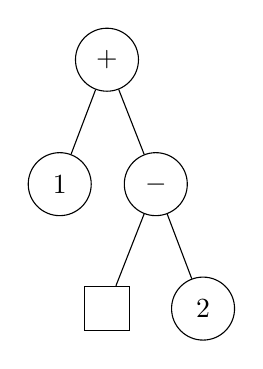
\begin{tikzpicture}[scale=0.02]
            \node [node] (1) at (51, 179) {$+$};
            \node [node] (2) at (21, 100) {1};
            \node [node] (3) at (82, 100) {$-$};
            \node [hole] (4) at (51,  21) {};
            \node [node] (5) at (112, 21) {2};

            \draw (1) -- (2);
            \draw (1) -- (3);
            \draw (3) -- (4);
            \draw (3) -- (5);
        \end{tikzpicture}
        \caption{Outside-in context}
    \end{minipage}
    \hfill
    \begin{minipage}{0.45\textwidth}
        \centering
        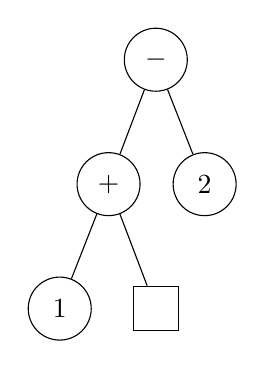
\begin{tikzpicture}[scale=0.02]
            \node [node] (1) at (51, 179) {$-$};
            \node [node] (2) at (21, 100) {$+$};
            \node [node] (3) at (82, 100) {2};
            \node [node] (4) at (-10, 21) {1};
            \node [hole] (5) at (51, 21)  {};

            \draw (1) -- (2);
            \draw (1) -- (3);
            \draw (2) -- (4);
            \draw (2) -- (5);
        \end{tikzpicture}
        \caption{Inside-out context}
    \end{minipage}
\end{figure}

%%%%%%%%%%%%%%%%%%%%%%%%%%%%%%%%%%%%%%%%%%%%%%%%%%%%%%%%%%%%%%%%%%%%%%%%%%%%%%%
\section{Programs, and Non-local Reductions: \texttt{call/cc}}

\begin{alignat*}{2}
  p & \Coloneqq e
    \tag{programs} \\
  e & \Coloneqq v \mid e\;e \mid \mathcal{K} x.e \mid \mathcal{A} p
    \tag{expressions} \\
  v & \Coloneqq x \mid v
    \tag{values}
\end{alignat*}

Thanks to evaluation contexts, we can define non-local control flow constructs.

\begin{alignat*}{2}
  E[\mathcal{K} x.e] & \longrightarrow E[e\{\lambda y.\mathcal{A} E[y] / x\}] \\
  E[\mathcal{A} p]   & \longrightarrow p
\end{alignat*}

%%%%%%%%%%%%%%%%%%%%%%%%%%%%%%%%%%%%%%%%%%%%%%%%%%%%%%%%%%%%%%%%%%%%%%%%%%%%%%%
\section{Further Reading}

As pointed out during the lecture, we've already seen one-hole contexts
on the Functional Programming course
in the data structure called \emph{The Zipper}~\citep{Huet97}.
Interestingly, \citet{McBride} observed that one-hole contexts used
in the Zipper data structure can be derived automatically,
and such a derivation has a lot in common with
a symbolic derivative of a function.
